\documentclass{article}
\usepackage{datetime, amsmath, xparse, graphicx, amssymb, geometry}
\geometry{margin=1.4in}
\usepackage{amsmath}
\DeclareMathOperator*{\argmax}{argmax}
% \usepackage[T1]{fontenc}

\title{Medical reports classification \\ \large Machine Learning}

\author{Hanna Nurska, 499866}

\newdateformat{monthyeardate}{\monthname[\THEMONTH], \THEYEAR}
\monthyeardate

\begin{document}
\maketitle
\begin{center}
    \textit{I affirm that this report is the result of my own work and that I did not share any part of it with anyone else except the teacher.}
\end{center}

\newpage

% \section{Introduction}

\section{Data analysis}
The dataset includes a total of 3331 medical reports divided into training set of size 2731, validation set of size 300 and test set of size 300. Each of the reports belong to one of 8 categories which are:
\begin{itemize}
    \item cardiovascular / pulmonary,
    \item consult,
    \item gastroenterology,
    \item general medicine,
    \item neurology,
    \item otthopedic,
    \item radiology,
    \item surgery.
\end{itemize}

The number of samples belonging to these classes are: 372 (cardiovascular / pulmonary), 355 (orthopedic), 223 (neurology), 516 (consult), 273 (radiology), 259 (general medicine), 1103 (surgery), 230 (gastroenterology) which is presented in figure \ref{fig:class_distr}.
\begin{figure}[!ht]
    \centering
    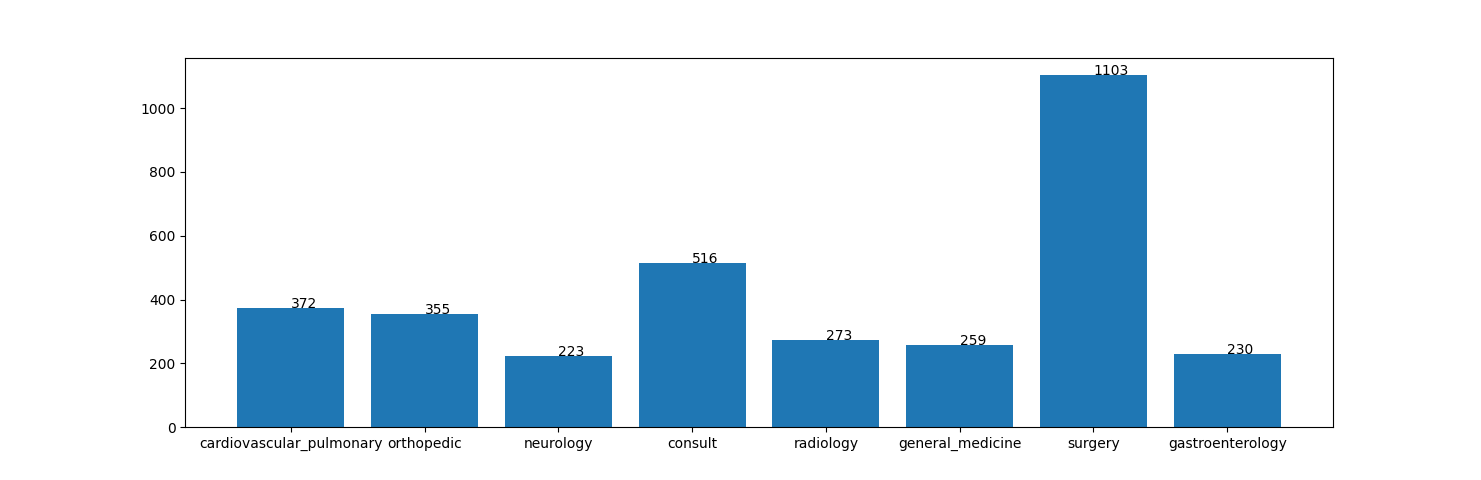
\includegraphics[width=\textwidth]{images/classes_distr.png}
    \caption{Class distribution}
    \label{fig:class_distr}
\end{figure}

The classes are distributed quite equally except class \textit{surgery} which has considerably more samples. When it comes to train set, number of samples from class \textit{surgery} also exceeds number of samples from other classes. The result is presented in figure \ref{fig:class_train_distr}. This might have influence on classification result, i.e. the class \textit{surgery} might be more probable to choose.

\begin{figure}[!ht]
    \centering
    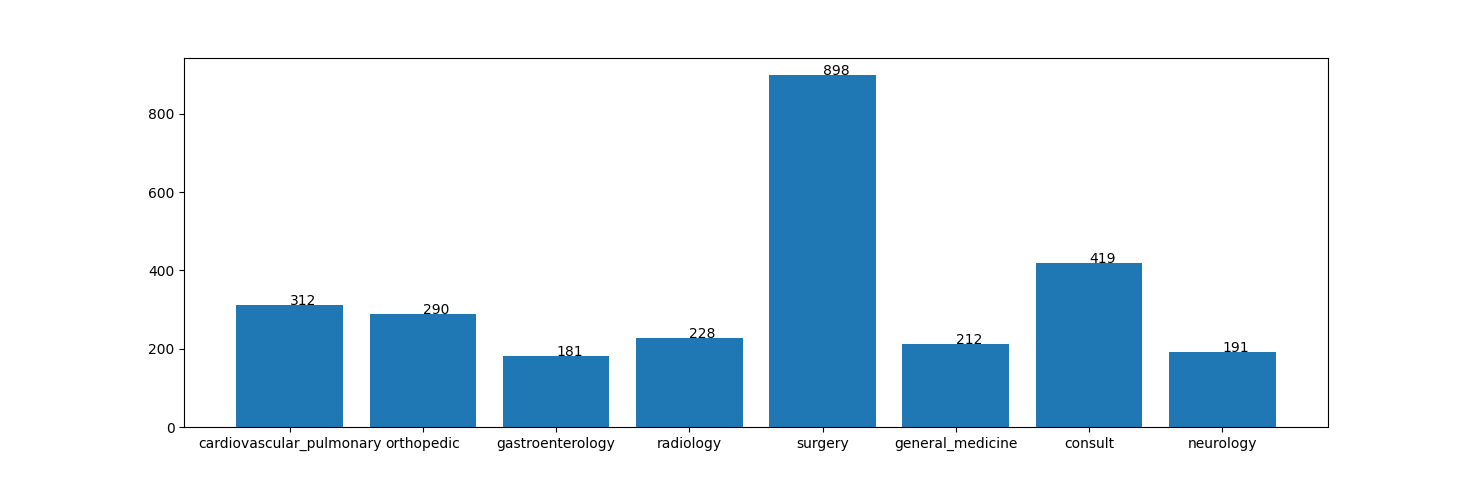
\includegraphics[width=\textwidth]{images/classes_train_distr.png}
    \caption{Class distribution}
    \label{fig:class_train_distr}
\end{figure}

The data is in format .txt, files contain plain text. In order to make use in classification model from this data, it is crucial to extract some features (for example number of occurances of the most popular words) as well as assigned class (we can derive it from the file name). The process and results of data extraction is described in section \ref{section:data_extraction}.


\section{Data extraction}
\label{section:data_extraction}
First of all, the \textit{n} most common words occuring in train data were derived and saved into \texttt{vocabulary.txt} file. The value \textit{n} was taken to be 2000. In order to get them, some text preprocessing was applied. To begin with, all punctuation and numbers were removed from the reports. Then, words shorter that 2 letters were deleted, as well as stopwords. Stopwords are words who are really common, which don't have influence on document identification. In other words, stopwords cannot help with recognising the nature of speech. Last but not least, all of the words were stemmed, which means that the endings of the words were cut off. The aim of this operation is to treat the same word in different gramatical forms as one word. The most common words in medical reports from train set were: \textit{patient, right, left, histori, us, place, procedure, normal, pain, year, ...}. As we can see, none of the 10 first words have nautral overtone, i.e. they don't indicate to which category of madicine they might refer. That's why it is important to choose as \textit{n} big enough value because a big part of common words will occur in many reports, regardless their categories.

After creating a vocabulary, it was used to redesign text reports into \textit{Bag of Words} representation. It's a representation which is a vector of the counters of the occurances of the most popular words (from \texttt{vocabulary.txt} file) in the text. The label of the sample was derived from its filename and then, transformed into a number. To do so, all of the classes were saved into a list and then, the index of the particular label was taken. The \textit{BoW} represantation of all of the reviews and their labels were later saved into a compressed file \texttt{train.txt.gz} The data normalization was not necessary since the features are only compared to each other.

At this stage, also validation and test data were converted into \textit{BoW} representation, normalised and saved into \texttt{valid.txt.gz} and \texttt{test.txt.gz}, respectively. Of course, the normalization applied to validation and test data was based on \textit{mean} and \textit{standard deviation} values derived from the training set.

For the data extraction part, the code developed in the lab activity was reused.

\section{Model selection}
Next step is selection of accurate classification model used for the training and after for the evaluation. In order to have wider perspective, two models were implemented, tried and tested. First of the models is Naive Bayes Classifier, described in more details in subsection\ref{subsection:naive_bayes}. As second model, Neural Network was tried out, which is described in subsection \ref{subsection:neural_network}.

\subsection{Multinomial Naive Bayes}
\label{subsection:naive_bayes}
Naive Bayes is an common model when it comes to text classification. In this approach, as well as in Neural Network approach, each word is treated as feature. The main assumption of Naive Bayes is that all of the features are conditionally independent which means that knowing a class of a sample, the knowledge about one of the features doesn't give any knowledge about any other feature.

In the task of classification of medical rewievs Multinomial model was used because there are more than two classes. The prediction of the Multinomial Naive Bayes is defined by the following formula:
\begin{equation}
    \hat{y} = \argmax_{y \in \{0, ..., k-1\}} \left( \sum^{n - 1}_{j = 0} x_j \log \pi_{y, j} \right) + \log P(y),
\end{equation}
where $x_j$ is the feature vector, $\pi_{y, j}$ is the learnt probability of the occurance the word $j$ in class $y$, $P(y)$ is the probability of the class $y$.

The main objective of the training is to find the probabilities $\pi_{y, j}$.



\subsection{Neural Network}
\label{subsection:neural_network}

\end{document}